\chapter{Beschreibung der verschiedenen Messungen und Ergebnisdarstellung}

\section{Konfiguration der Router}
Die folgenden Schritte sind bei allen Routern durchzuf�hren.
\subsection{Basiskonfiguration}
Zun�chst ist der Hostname zu R1 zu �ndern. Anschlie�end werden die Passw�rter
konfiguriert und ``logging synchronous'' aktiviert.
\begin{lstlisting}
Router>enable
Router#configure terminal
Router(config)# hostname R1
R1(config)#line console 0
R1(config-line)#password cisco
R1(config-line)#login
R1(config-line)#exit
R1(config)#line vty 0 4
R1(config-line)#password cisco
R1(config-line)#login
R1(config)#enable password cisco
R1(config)#enable secret class
R1(config)#exit
R1(config)#line console 0
R1(config-line)#logging synchronous
\end{lstlisting}
F�r die Konsole wird das Passwort ``cisco'', f�r den Priviledged EXEC Mode
``class'', vergeben. Durch ``logging synchronous'' wird sichergestellt, dass
keine Systemnachrichten die Befehlseingabe unterbrechen.
\newline
Um die Weiterleitung von IPv6-Paketen zu erm�glichen, muss im \acs{CLI} des
Routers das Kommando \textit{ipv6 unicast-routing} ausgef�hrt werden.
\newline
Router 2 und Router 3 werden �uivalent konfiguriert.

\subsection{Fast-Ethernet-Schnittstelle}\label{FE}
Im Configuration Mode wird die Fast-Ethernet-Schnittstelle 0/0 konfiguriert und
die entsprechende IPv6-Adresse, sowie die Link-Local-Adresse, aus \ref{config1}
zugewiesen:
\begin{lstlisting}
R1(config)#interface FastEthernet 0/0
R1(config-if)#description R1 LAN Default Gateway
R1(config-if)#R1(config-if)# ipv6 address 2001:DB8:1:1::1/64
R1(config-if)# ipv6 address FE80::1 link-local
R1(config-if)#no shutdown
R1(config-if)#exit
R1(config)#exit
\end{lstlisting}
\subsection{Serial-Schnittstelle}
Analog zu \ref{FE} wird die Serial-Schnittstelle 0/0 konfiguriert:
\begin{lstlisting}
R1(config)#interface serial 0/0/0
R1(config-if)#description WAN link to R2
R1(config-if)#ipv6 address 2001:DB8:1:A001::1/64
R1(config-if)#clock rate 64000
R1(config-if)#no shutdown
R1(config-if)#exit
R1(config)#exit
\end{lstlisting}

\section{Konfiguration der Hosts}
Den Hosts wird das jeweilige Default Gateway (Link-Local-Adresse) und die
entsprechende statische IPv6-Adresse gem�� \ref{config1} zugewiesen. 
%TODO erkl�ren?

\section{�berpr�fung der Konfiguration}

\subsection{�berpr�fung mittels Ping-Befehlen}
Zun�chst wird mittels Eingabeaufforderung �berpr�ft, ob die Konfiguration der
Hosts korrekt ist.\footnote{siehe Anhang \ref{ipconfig}}
\newline
Danach werden Ping-Befehle ausgef�hrt um die Konfiguration zu testen:
\begin{itemize}
  \item PC1 zu R1
  \item PC2 zu R2
  \item PC3 zu R3
\end{itemize}
Die Befehle verlaufen alle erfolgreich.\footnote{siehe Anhang \ref{pingrouter}}

\subsection{IPv6 Einstellungen}
Durch \textit{show ipv6 interface brief} l�sst sich der Status der Interfaces
�berpr�fen:
\begin{lstlisting}
R1#sh ipv6 interface brief
FastEthernet0/0            [up/up]
    FE80::1
    2001:DB8:1:1::1
FastEthernet0/1            [administratively down/down]
Serial0/0/0                [up/up]
    FE80::290:2BFF:FE95:C001
    2001:DB8:1:A001::1
Serial0/0/1                [administratively down/down]
Vlan1                      [administratively down/down]
\end{lstlisting}

Bei der Fast-Ethernet-Schnittstelle 0/0 werden zwei IPv6-Adressen angezeigt, die
Link-Local-Adresse und die zuvor konfigurierte IP-Adresse der Schnittstelle.
%TODO kind of IP-Addresses

\begin{lstlisting}
R1>show ipv6 interface
FastEthernet0/0 is up, line protocol is up
  IPv6 is enabled, link-local address is FE80::1
  No Virtual link-local address(es):
  Global unicast address(es):
    2001:DB8:1:1::1, subnet is 2001:DB8:1:1::/64
  Joined group address(es):
    FF02::1
    FF02::2
    FF02::1:FF00:1

  [...]
\end{lstlisting}
Bei Router 1 werden drei Multicast-Adressen angezeigt.
\newline
Die folgende Abbildung zeigt das Format einer IPv6-Multicast-Adresse:
\begin{figure}[ht]
  \centering
     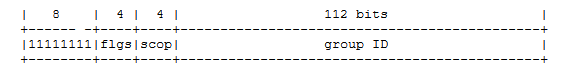
\includegraphics[width=\linewidth]{Graphics/multicast_frame.PNG}
  \caption{Format einer IPv6 Mulicast-Adresse}
  \label{fig:multicast}
\end{figure}

Der Scope ist bei allen aufgef�hrten Adressen 2, d.h. es handelt sich um einen
Link-Local Multicast-Scope.\cite[13]{RFC4291}
\newline
FF02::1 adressiert alle IPv6-Hosts. Diese Adresse ist vergleichbar mit der
Broadcast-Adresse bei IPv6.
\newline
FE02::2 adressiert alle Router.
\newline
Die dritte aufgef�hrte Multicast-Adresse ist eine Solicited-Node-Adresse.
%TODO erkl�ren? welche adresse ist das??
\subsubsection{Solicited-Node-Adressen}\label{solicited}
Die in der Versuchsanleitung sind zwei weitere Multicast-Adressen
genannt:\footnote{siehe Versuchsanleitung S.14}
\begin{itemize}
  \item FF02::1:FF00:1
  \item FF02::1:FF0D:1A60
\end{itemize}
Es handelt sich um sog. ``Solicited-Node''-Adressen.\parencite[15]{RFC4291}
\newline
Solicited-Node-Adresse sind Multicast-Adressen, die aus Unicast- und
Anycast-Adresse des PCs gebildet werden. Die niederwertigsten 24 Bit der
Unicast-oder Anycast-Adresse werden dem 104 Bit langem Pr�fix
(FF02:0:0:0:0:1:FF00::/104) angeh�ngt. Dadurch ergibt sich folgender
Wertebereich:\cite{RFC4291}\cite{RFC2461}
\newline
FF02:0:0:0:0:1:FF00:0000 bis
FF02:0:0:0:0:1:FFFF:FFFF
\newline
Solicited-Node-Adressen werden beim \ac{NDP} verwendet.\cite{RFC2461}

\section{Konfiguration von IPv6-Routing}

\subsection{Statische Routen}
Zun�chst wird eine statische Route von Router 1 zu Router 2 konfiguriert,
ausgehend von der Serial-Schnittstelle 0/0/0.

\begin{lstlisting}
R1(config)#ipv6 route 2001:DB8:1:2::1/64 Serial 0/0/0
\end{lstlisting}

Anschlie�end existiert ein entsprechender Eintrag in der Routingtabelle von
Router 1:

\begin{lstlisting}
R1#sh ipv6 route
IPv6 Routing Table - 6 entries
Codes: C - Connected, L - Local, S - Static, R - RIP, B - BGP
       U - Per-user Static route, M - MIPv6
       I1 - ISIS L1, I2 - ISIS L2, IA - ISIS interarea, IS - ISIS summary
       O - OSPF intra, OI - OSPF inter, OE1 - OSPF ext 1, OE2 - OSPF ext 2
       ON1 - OSPF NSSA ext 1, ON2 - OSPF NSSA ext 2
       D - EIGRP, EX - EIGRP external
C   2001:DB8:1:1::/64 [0/0]
     via ::, FastEthernet0/0
L   2001:DB8:1:1::1/128 [0/0]
     via ::, FastEthernet0/0
S   2001:DB8:1:2::/64 [1/0]
     via ::, Serial0/0/0
C   2001:DB8:1:A001::/64 [0/0]
     via ::, Serial0/0/0
L   2001:DB8:1:A001::1/128 [0/0]
     via ::, Serial0/0/0
L   FF00::/8 [0/0]
     via ::, Null0
\end{lstlisting}
\subsection{Default Routen}
Alle statischen Routen werden entfernt:
\begin{lstlisting}
R1(config)#no ipv6 route 2001:DB8:1:2::1/64 Serial 0/0/0
\end{lstlisting}
Danach wird eine Deafult-Route angelegt:
\begin{lstlisting}
R1(config)#ipv6 route ::/0 Serial 0/0/0
\end{lstlisting}

Die Routingtabelle von Router 1 enth�lt anschlie�end die neu konfigurierte
Route:
\begin{lstlisting}
R1#show ipv6 route
IPv6 Routing Table - 6 entries
Codes: C - Connected, L - Local, S - Static, R - RIP, B - BGP
       U - Per-user Static route, M - MIPv6
       I1 - ISIS L1, I2 - ISIS L2, IA - ISIS interarea, IS - ISIS summary
       O - OSPF intra, OI - OSPF inter, OE1 - OSPF ext 1, OE2 - OSPF ext 2
       ON1 - OSPF NSSA ext 1, ON2 - OSPF NSSA ext 2
       D - EIGRP, EX - EIGRP external
S   ::/0 [1/0]
     via ::, Serial0/0/0
C   2001:DB8:1:1::/64 [0/0]
     via ::, FastEthernet0/0
L   2001:DB8:1:1::1/128 [0/0]
     via ::, FastEthernet0/0
C   2001:DB8:1:A001::/64 [0/0]
     via ::, Serial0/0/0
L   2001:DB8:1:A001::1/128 [0/0]
     via ::, Serial0/0/0
L   FF00::/8 [0/0]
     via ::, Null0
\end{lstlisting}


%TODO NDP
%FF02::1:FF00:F destination im ndp paket
%TODO RIP